\documentclass[10pt,oneside,openany]{brownthesis}
\usepackage{times}
\usepackage{latexsym}
\usepackage{url}
\usepackage{multirow}
\usepackage{amssymb}
\usepackage{amsmath}
\usepackage{algpseudocode}
\usepackage{graphicx}

% All package includes, setup, and general-purpose command definitions are contained in prelude.tex
% Redefines / Overrides the 'book' document class's default chapter heading formatting
\makeatletter
\def\@makechapterhead#1{%
  \vspace*{50\p@}% <----------------- Space from top of page to Chapter #
  {\parindent \z@ \raggedright \normalfont
    \ifnum \c@secnumdepth >\m@ne
        \Huge\bfseries \@chapapp\space \thechapter% <-- Chapter #
        \par\nobreak
%        \vskip 20\p@% <-------------- Space between Chapter # and title
    \fi
    \interlinepenalty\@M
    \huge \textit{#1}\par\nobreak% <------------------ Chapter title
    \vskip 40\p@% <------------------ Space between chapter title and first paragraph
  }}
\makeatother


\usepackage[margin=1in]{geometry}

%%%% Includes for Minion %%%%%
\usepackage[T1]{fontenc}
%\usepackage[lf]{MinionPro}
%\usepackage{MnSymbol}
%\usepackage{MyriadPro}
\usepackage{inconsolata} % nicer tt font

\usepackage{lipsum} % Provides \lipsum command for generating random text
\usepackage{setspace} % Provides \doublespacing command for double spacing
\usepackage[utf8]{inputenc} % Generally useful UTF-8 characters
\usepackage[tracking=true,activate={true,nocompatibility},final,kerning=true,spacing=true]{microtype}% Drastically improves character and line spacing and wrapping
%\DisableLigatures{encoding = *, family = * } % This is useful for copy/paste with no ligatures
\usepackage{xcolor} % For defining colors
\usepackage{xspace} % The \xspace command conditionally adds spaces
\usepackage{cite} % Numerically orders multiple citations and shrinks 2,3,4 into 2-4
\usepackage{paralist} % Provides compactitem
\usepackage{graphicx} % Fundamental package for \includegraphics
\usepackage{caption} % Provides control over caption fonts and spacing
\usepackage{subcaption} % For subfigure environment
\usepackage{tabu} % Tabu is a decent package for more customizable tables
\usepackage{makecell} % Helpful cell alignment package for tabu
\usepackage[usestackEOL]{stackengine} % \shortstack command with configurable line spacing
\usepackage{enumitem} % adds spacing options for itemize and enumerate
\usepackage{pifont} % provides the circles with numbers inside them
\usepackage{stmaryrd} % provides \shortrightarrow and other symbols
\usepackage{relsize} % provides \relsize command to reduce text size relative to current size
\usepackage{adjustbox} % for rotating text
\usepackage{array} % provides bottom alignment in tables
\usepackage{multirow} % span multiple rows in tables
\usepackage{verbatimbox} % create verbatim boxes and use them in tables
\usepackage{layouts} % lets you print various widths like \columnwidth
\usepackage{bm} % Bold math 
\usepackage{epigraph} % quotationas at the beggining of sections
\usepackage[hang,flushmargin]{footmisc} % Footnote options such as spacing
\usepackage{listings} % code listings
\usepackage{ stmaryrd }
\usepackage[titletoc,title]{appendix}
\usepackage{amsthm} % Provides proof environment

\usepackage[most]{tcolorbox} % provides good color boxes, \tcolorbox, which is better than xcolors colorbox
\tcbuselibrary{breakable}

% Tikz drawing package and a bunch of libraries that add functionality
\usepackage{tikz}
\usetikzlibrary{arrows}
\usetikzlibrary{arrows.meta}
\usetikzlibrary{bending}
\usetikzlibrary{intersections}
\usetikzlibrary{decorations.markings}
\usetikzlibrary{fadings}
\usetikzlibrary{decorations.pathmorphing}
\usetikzlibrary{decorations.text}
\usetikzlibrary{shapes.geometric}
\usetikzlibrary{decorations.pathreplacing}
\usetikzlibrary{calc}
\usetikzlibrary{fit}
\usetikzlibrary{patterns}
\usetikzlibrary{plotmarks}
\usetikzlibrary{trees}
\usetikzlibrary{backgrounds}
\usetikzlibrary{positioning}
\usepackage{algorithm2e}

%%%% Includes for URLs and links between section in doc %%%%%
\definecolor{figurecolor}{RGB}{22,90,220}
\definecolor{citecolor}{RGB}{198,81,19}
\usepackage{url}
\usepackage[pdftex,colorlinks,pdfusetitle]{hyperref} % References are links; use \title and \author for pdf title and author
\usepackage[hyperpageref]{backref}
\usepackage[nameinlink,noabbrev]{cleveref} % Does the automatic referencing malarky (eg, "figure")
\DeclareCaptionLabelSeparator{forcespace}{~} % Fixing a subcaption spacing bug
\captionsetup[subfigure]{labelsep=forcespace}
\captionsetup[figure]{labelfont={color=figurecolor}}
\captionsetup[table]{labelfont={color=figurecolor}}
%\renewcommand*{\backref}[1]{% for backref < 1.33 necessary
%\renewcommand*{\backrefalt}[4]{\ifcase #1 \or (\S #2). \else (\S #2). \fi}
\renewcommand*{\backrefalt}[4]{\ifcase #1 \or Page #2. \else Pages #2. \fi}
\renewcommand\thefootnote{{\textcolor{citecolor}{\arabic{footnote}}}}
\hypersetup{
	colorlinks=true,
	urlcolor=black,
	linkcolor=figurecolor,
	citecolor=citecolor,
	pdfstartview=FitH %,
}

% automatically use the \S symbol for section autoref and eat the space
\def\Snospace~{\S{}}
\renewcommand*\sectionautorefname{\Snospace}
\renewcommand*\subsectionautorefname{\Snospace}
\renewcommand*\subsubsectionautorefname{\Snospace}
\renewcommand*\chapterautorefname{Chapter}
\newcommand{\lstnumberautorefname}{Line}
\renewcommand*\algorithmautorefname{Algorithm}
%%%%%%%%%%%%%%%%%%%%

\frenchspacing % Single-spaced sentence spacing

\usepackage{expl3}
\ExplSyntaxOn
\newcommand\latinabbrev[1]{
  \peek_meaning:NTF . {% Same as \@ifnextchar
    #1\@}%
  { \peek_catcode:NTF a {% Check whether next char has same catcode as \'a, i.e., is a letter
      #1.\@ }%
    {#1.\@}}}
\ExplSyntaxOff
\def\etc{\latinabbrev{etc}}

\newcommand{\eg}{\emph{e.g.}\xspace}
\newcommand{\cf}{{cf.}\xspace}
\newcommand{\ie}{\emph{i.e.}\xspace}
\newcommand{\etal}{\emph{et al.}\xspace}

\newcommand{\fakepara}[1]{\vspace{0.2em}\noindent\textbf{#1}\ \ }


% Styles the \url command to have less spacing between characters
% zi4 is the inconsolata font
\SetTracking[spacing={-50*,0*,50*}]{encoding=T1, family=zi4}{-40}
\renewcommand\UrlFont{\fontfamily{zi4}\lsstyle}
%\Urlmuskip=-1mu\relax

% Style smallcaps spacing
\SetTracking{encoding={T1}, shape=sc}{-10}

% Shorter underscore character
\newcommand{\smallunderscore}{\rule{0.75ex}{.4pt}}

\begin{document}
\newcommand{\thesistitle}{Cross-Document Coreference Resolution for Entities and Events}
\author{Chris Tanner}
\title{\thesistitle\\~\\ Ph.D. Thesis Proposal \\ (draft as of April 19, 5pm)}
\date{May 16, 2018}

\frontmatter % PROPOSAL

\maketitle % PROPOSAL

\mainmatter % PROPOSAL

%\doublespacing

\def\abstract#1{\gdef\d@abstract{#1}}
\def\d@abstract{}
\def\abstractpage{%
  \thispagestyle{empty}
  \noindent Abstract of ``\thesistitle''
  \\
  % The dissertation must be accompanied by an abstract which will be published
% in Dissertation Abstracts International. The abstract should, in a concise
% manner, present the problem of the dissertation, discuss the materials and
% procedure or methods used, and state the results or conclusions. Mathematical
% formulas, diagrams, and other illustrative materials should be avoided. The
% abstract should not be part of the dissertation itself nor should it be
% included in the table of contents. The abstract should be presented in two
% unnumbered loose copies. It should be headed as follows:
% 
% Abstract of (TITLE OF DISSERTATION), by (AUTHOR'S NAME), Ph.D., Brown
% University, May (YEAR IN WHICH DEGREE IS TO BE AWARDED).
% 
% The abstract should be prepared carefully since it will be published without
% editing or revision. The abstract should be double-spaced and may not exceed
% 350 words (maximum 2,450 typewritten characters — including spaces and
% punctuation — about 70 characters per line with a maximum of 35 lines). If
% the 350-word limit is exceeded, University Microfilms will simply cut off the
% abstract at this point.
Abstract Here
  \vfill}
\abstractpage
{
\singlespacing
\hypersetup{linkcolor=black}
\tableofcontents % PROPOSAL
\doublespacing
}
%\listoffigures 
%\listoftables
\chapter{Introduction}
\input{introduction}

\chapter{Related}
\input{Related}

\chapter{Corpora}
\label{sec:corpus}
Annotating a corpus with coreference information is an expensive task, as every sentence should include at least one entity and event.  Since many of these mentions will refer to other mentions in the same sentence, document, or other documents, the task quickly becomes complex and time-consuming.  Further, many mentions can be tricky to perfectly annotate, and consequently, annotators will often differ in their markings.  Therefore, multiple annotators label every sentence, allowing a majority vote to resolve discrepancies.  Due to these difficulties, there are not many event corpora, yet the ECB+ is sufficient for research, and we now describe its evolution.

\section{Event Coreference Corpora}
\subsection{ECB: EventCorefBank}
Created by Bejan and Harabagiu in 2010 \cite{Bejan:2010:UEC:1858681.1858824}, the ECB corpus provides within-document and cross-document event coreference annotations for 480 documents, spanning 43 disjoint \textit{topics}.  The documents were selected from GoogleNews archive\footnote{http://news.google.com} and each topic is a collection of documents (roughly 7-15 relatively short documents) which all concern the same seminal event, such as a particular arrest, transaction, attack, sporting event, election, etc.  Each event mention, and its relation with another event, was annotated, where an even relation is one of six types: subevent, reason, purpose, enablement, precendence, and related.  The weakness of this corpus is that (1) only a subset of the sentences were annotated; (2) only events were annotated -- no entities.

\subsection{EECB: Extended ECB}
Lee, et. al. \cite{Lee:2012:JEE:2390948.2391006} extended the ECB corpus by addressing both of the aforementioned weaknesses; four annotators fully annotated all sentences, with entity coreference relations included.  Also, they removed the originally-annotated relations, only keeping the coreference ones (e.g., subevent, purpose, related).  Note, \textit{light verbs} were not annotated (e.g., \textit{make} an offer or \textit{give} a talk).

\subsection{ECB+: EventCorefBank+}
All of our event-based experiments were conducted on this corpus, as it is the largest and commonly used corpus.  It includes the 480 documents from the original ECB corpus, along with 502 additional documents which stem from 43 additional topics which are highly similar to the original 43 topics from the original ECB corpus.  For example, Topic 1 in the ECB corpus contains documents which concern Tara Reid checking into a rehab center in Malibu, California.  However, Topic 1 in the ECB+ corpus also includes documents which concern Lindsay Lohan checking into a rehab center in Rancho Mirage, California.  The purpose for this similarity is to help create a more realistic and potentially confusable scenario for the cross-document task.  However, it has been shown \cite{journals/tacl/YangCF15} that one can simply perform document classification as a pre-processing step, which will allow a cross-document model to appropriately, perfectly confine itself to a relevant document set from which to consider linking mentions (e.g., ECB's Topic 1 documents can be easily separable from ECB+'s added Topic 1 documents).

We maintain the same train/dev/test splits as previous researchers, as further detailed in Chapter \ref{sec:coreference}.  A sample of the corpus in shown in Figure \ref{fig:corpus}, and statistics are listed in Table \ref{tab:ECB1}, where it is clear that the majority of gold mentions are one token in length (e.g, \textit{announced}).  \textbf{NOTE:} the corpus contains 15,812 sentences.  The corpus creators only place stock in their annotations for 1,840 specific sentences.  However, they also annotate some additional sentences which they place less stock in (e.g., not all annotators labelled these additional sentences).  All research papers which use this corpus simply evaluate again all labelled mentions, even if they do not belong to the well-supported 1,840 sentences.  For fair comparison, we follow suit.

\begin{table}
\centering
\begin{tabular}{c|c|c|c|c|}
\cline{2-5}
& Train & Dev & Test & Total \\ \cline{1-5} \hline
\multicolumn{1}{ |c| }{\# Documents} & 462 & 73 & 447 & 982   \\ %\cline{1-5}
\multicolumn{1}{ |c| }{\# Sentences} & 7,294 & 649 & 7,867 & 15,810    \\ 
\multicolumn{1}{ |c| }{\# Mentions-1} & 1,938 & 386 & 2,837 & 5,161    \\ %\cline{1-5}
\multicolumn{1}{ |c| }{\# Mentions-2} & 142 & 52 & 240 & 434    \\ %\cline{1-5}
\multicolumn{1}{ |c| }{\# Mentions-3} & 18 & -- & 25 & 43    \\% \cline{1-5}
\multicolumn{1}{ |c| }{\# Mentions-4} & 6 & -- & 7 & 13   \\ \cline{1-5}
\end{tabular}
\caption{Statistics of the ECB+ Corpus, where Mentions-N represents event mentions which are N-tokens in length.}
\label{tab:ECB1}
\end{table}


%\section{Entity Coreference Corpora}
%Forthcoming

\chapter{Event Coreference Resolution}
\label{sec:coreference}

Our current work has primarily focused on event coreference resolution.

\section{Initial Approaches}
Our initial approaches were unsuccessful but largely informative: we tried modelling all mentions (cross-document) at the same time, in a \textit{mention-pair} manner.  Given $N$ mentions in a given topic, we evaluated $\frac{N*(N-1)}{2}$ mention pairs, with the aim of predicting which were coref or not (i.e., a 0 or 1 prediction).  Approximately 1 out of every 15 mention pairs are actually co-referenced (gold truth).  Our supervised, classification modelling attempts included using various LSTM and SVM approaches.


\textbf{LSTMs:} The LSTM approaches were based on the fact that if we let $m_{i-1}$ represent the word immediately before mention $m_{i}$ in the corpus, then $m_{i-1}$ will have high likelihood of predicting $m_{i}$.  Our idea was that if $m_{i-1}$ has high likelihood of also predicting mention $m_{j}$, then $m_{j}$ and $m_{i}$ might be coreference.  Our premise was that the likelihood of predicting each mention is directly correlated with each mention's likelihood of referring to the same event as $m_{i}$.  Despite many attempts, this never gave good results.  My conclusions were that:

\begin{itemize}
\item LSTMs are sensitive and are too close to memorizing the exact sequence of words, especially given the variance in our corpus
\item Our corpus' context varies too much and is not conducive to our premise.  For example, one sentence may be ``Barack Obama \textit{spoke} ... '' and another sentence may be ``The President, on Tuesday, \textit{spoke} ...''.  The word Tuesday is not likely to predict the word \textit{spoke}.
\end{itemize}

\textbf{SVMs:} Our SVM approach used a variety of commonly-used lexical features.  The performance exceeded the \textit{SameLemma} baseline.  However, difficulties included the class imbalance (too many negatives examples per positive example), along with the computational expense of training a proper kernel -- yielding the model intractable.

We also tried a generative, \textbf{topic modelling} approach, a la LDA with Gibbs sampling.  The underlying event was our latent variable: P(Event|Document) and P(Mention|Event).  Again, our performance barely rivalled the baseline of \textit{SameLemma}.  My conclusion was that predicting the number of latent classes (traditionally, number of topics) is too difficult and drastically affects the performance, especially since nearly half of all events only have 1 mention.

From these attempts, along with the two previously published works which have used a ECB+ corpus \cite{journals/tacl/YangCF15, Choubey2017EventCR}, I drew the following conclusions:
\begin{itemize}
\item an event-level model is not ideal, since it is inappropriate to predict how many unique events exist
\item negative sub-sampling is critical
\item most importantly, predicting within-document links first is critical and easier, as there are fewer mentions, and it serves as a stepping stone before considering links across all documents.  Then, one can use these predicted within-document clusters to merge with other within-doc clusters that reside in other documents. 
\end{itemize}

\section{CCNN: Conjoined Convolutional Neural Network}
Conjoined Neural Networks (a.k.a. Siamese Networks) were first introduced by Bromly and LeCun \cite{SiameseNet} for the task of determining if two signatures were from the same person or not.  Specifically, Conjoined Networks are two identical neural networks, each of which accepts distinct inputs, which are joined by a single loss function over their highest-level features.  The loss function computes a similarity score (e.g., euclidean distance) for an input pair.  The networks are said to be conjoined because they share the same weights and thus work together as one network that learns how to discriminate.  The benefits of tying the weights are that it:
\begin{enumerate}
\item Ensures that similar inputs will be mapped appropriately, otherwise, they could be mapped to hidden representations that are dissimilar from their input representations; and
\item Forces the network to be symmetric. If we abstractly represent the Conjoined Network as a function, then:
$CCNN(f_i,f_j) \equiv CCNN(f_j,f_i)$.  This is critical, as the CCNN's similarity function should be independent of the ordering of its input pair.
\end{enumerate}

Last, Conjoined Networks have been shown to perform well in low-resource situation \cite{Koch2015SiameseNN}.  This is ideal for our task, as it is highly likely that at test time we encounter event mentions that are out-of-vocabulary (OOV).  We desire our model to discriminately learn the relationships of input mentions, rather than exclusively relying on the input values themselves.  Likewise, we choose to use a Convolutional Network due to:
\begin{enumerate}
\item their power in learning sub-regions of features and the relations thereof, and
\item their recent advances in many NLP tasks \cite{DBLP:conf/emnlp/Kim14,DBLP:conf/acl/GehringAGD17,DBLP:journals/corr/YuV17}.
\end{enumerate}

\subsection{Input Features}
\label{sec:features}
Since our CCNN needs each mention to be represented exclusively by its own input, we used none of the relational features\footnote{We also experimented with extending our CCNN model by adding relational features as a merged-layer at the highest neural level.} that are common in other coreference systems (e.g., SameLemma, Jaccard similarity of mentions' context, shared WordNet parents).  We used Stanford CoreNLP \cite{manning-EtAl:2014:P14-5} to extract the following features, which we thoroughly tested in different ways:
\begin{itemize}
  \item \textbf{Part-of-Speech:} LSTM-learned POS embeddings; and 1-hot representations.
  \item \textbf{Lemmatization}: Lemmatized each token and represented it by pre-trained GloVe \cite{pennington2014glove} word embeddings.
  \item \textbf{Dependency Lemma:} we represent the dependent parent/children of each token via their aforementioned lemma embeddings.
  \item \textbf{Character Embeddings:} each token is represented as a concatenation of its character embeddings.
  \item \textbf{Word Embeddings:} pre-trained GloVe word embeddings.
\end{itemize}
We account for mentions' having varying token lengths by summing their tokens in place, thus representing each mention as a fixed-length vector.

\subsection{Architecture}
We define the full embedding for a given token $t$ as $t_{emb} = t_{f_{1}} \oplus t_{f_{2}} \oplus \ldots \oplus t_{f_{n}},$ where $\oplus$ represents vector concatenation and $t_{f_{i}}$ represents a specific input feature vector.

Naturally, we may want to convolve over the context of mention $m$, too, by including the $N$ words before and after $m$.  Thus, our input for mention $m$ is a matrix $M$, and a la Kim \cite{DBLP:conf/emnlp/Kim14}, we zero-pad unfilled windows.

\vspace{3mm}

Let $\textbf{M}$ represent the full matrix corresponding to mention $m$: $\textbf{M} \in \mathbb{R}^{(2N+1) \times d}$ and $\textbf{M}_{(i,j),(k:l)}$ represent the sub-matrix of $M$ from $(i,j)$ to $(k,l)$.

\vspace{3mm}

We define a kernel with dimensions $(h,w)$, where $h < (2N+1)$ and $w < d$.  This allows the kernel to operate on sub-sections of the embeddings.  The kernel has an associated weight matrix $\textbf{w} \in \mathbb{R}^{h \times w}$.  Starting at a given index $(i,j)$ within mention matrix $\textbf{M}$, a feature $c_{i}$ is defined as:
\begin{equation}
c_{i} = f(\textbf{w}^{T}\textbf{M}_{(i:i+h-1),(j:j+w-1)} + b)
\end{equation}
where $b \in \mathbb{R}$ is an added bias term.  The kernel runs over every possible sub-section of mention matrix $\textbf{M}$, yielding a feature map $\textbf{c} \in \mathbb{R}^{(2N-h) \times (d-w-1)}$

\vspace{3mm}

Since the network is comprised of two identical, conjoined halves, we sufficiently represent the architecture in Figure \ref{fig:ccnn} with just one half.  The Lambda function calculates the Euclidean distance of each half's univariate vector and emits a two-class softmax prediction regarding the likelihood of the two mentions being co-referent.

\begin{figure*}[h]
\centering
	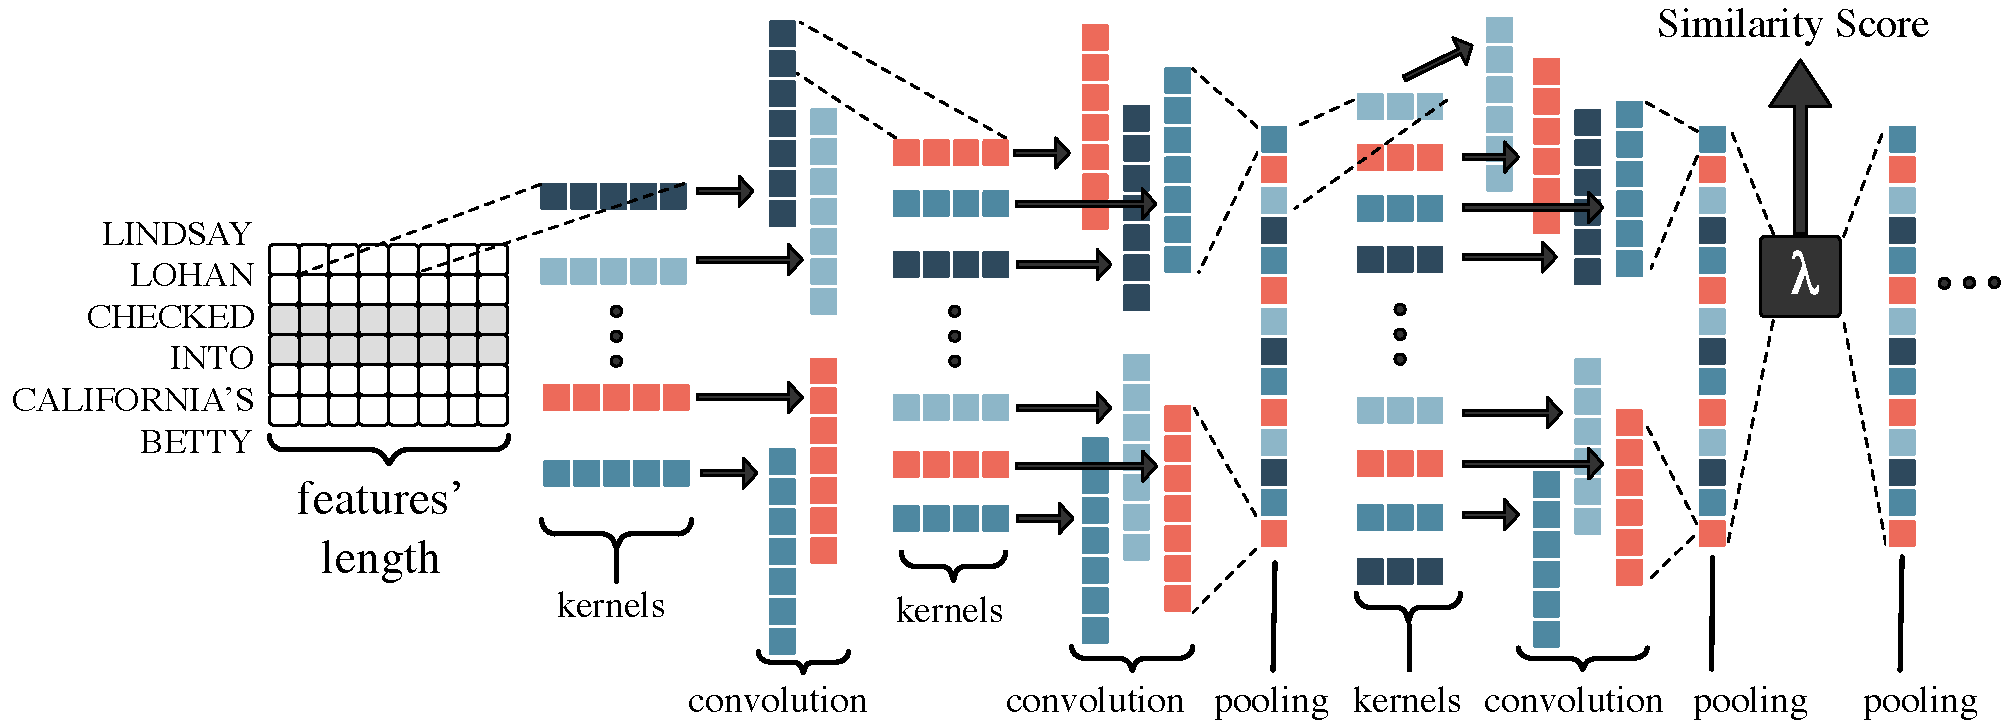
\includegraphics[width=1\textwidth]{graphics/architecture.pdf}
	\caption{One half of the Conjoined Convolutional Neural Network's Architecture.}
	\label{fig:ccnn}
\end{figure*}

\subsection{Loss / Optimization}
Our goal is to maximize discriminability of different event mentions, while enforcing features to be as similar as possible when they are of the same event.  Contrastive Loss, shown in Equation \ref{eq:contrastive}, is perfectly suited for this objective \cite{SchroffKP15,pmlr-v48-liud16}. Our training set has a strong class imbalance (most input pairs are not co-referent), so we down-sample to a 5:1 ratio of negative-to-positive examples.  We use Adagrad for optimization.
\begin{equation}
\begin{aligned}
L(&\hat{y},y)=\frac{1}{2N}\sum_{n=1}^{N}[(y)d^2 + (1-y)*(max(1-d,0))^2] \\
&\textnormal{where }d=\|y_{n}-\hat{y}_{n}\|_{2}
\end{aligned}
\label{eq:contrastive}
\end{equation}


%%%%%%%%%%%%%%%%%%%%%%%%%%%%%%%%%%%%%%%%%%%%%%%%%
%%%%%%%%%%%%%                5.   NEURAL CLUSTERING                %%%%%%%%%%%%%%%
%%%%%%%%%%%%%%%%%%%%%%%%%%%%%%%%%%%%%%%%%%%%%%%%%

\section{Neural Clustering (NC)}
\label{sec:clustering}
It is common practice for mention-pair models to first assign a probability score to every mention-pair, and then cluster with a different model.

\subsection{Existing Clustering Approaches}
\textbf{Agglomerative Clustering} is a simple but effective approach.  It first assigns each mention to its own singleton cluster.  Then, it repeatedly merges the two distinct clusters which contain the shortest-distance mention pairs.  Although this is a strong baseline, as seen in Yang, et. al. \cite{journals/tacl/YangCF15}, there are three main weaknesses:
\begin{enumerate}
\item One must define a stopping threshold $\alpha$.
\item Any given $\alpha$ hinges on the data being uniform across documents.  In reality, distances between mention-pairs could vary significantly between documents and topics.
\item Most significant, each cluster merge is based solely on two individual mentions, yet these mentions may not be representative of the cluster at large.
\end{enumerate}

\textbf{HDDCRP and Iterative-Folding Clustering} both contain the issue \#3 from above, as detailed in Sections \ref{sec:HDDCRP} and \ref{sec:Choubey}.

\subsection{Our Approach}
We aim to use the strengths of agglomerative clustering, while replacing its shortcomings.  We train a classifier to learn the most likely {positive cluster merge}, where the cluster is represented more holistically than a mention-pair basis.

Specifically, we learn a function $f(C_x,C_y)$ that predicts the likelihood of an appropriate, positive merging of clusters $(C_x,C_y)$. Let $d(m_i,m_j)$ be the mention-pair distance predicted by our CCNN model, where $m_i \in C_x$, and $m_j \in C_y$.  Function $f(C_x,C_y)$ is based on four simple features:
\begin{itemize}
  \item min-pair distance: $\min_{m_i,m_j} d(m_i,m_j)$
  \item avg-pair distance: $\frac{\sum_{m_i, m_j} d(m_i,m_j)}{\|C_x\|\|C_y\|}$
  \item max-pair distance: $\max_{m_i,m_j} d(m_i,m_j)$
  \item size of candidate cluster: $\frac{\|C_x\| + \|C_y\|}{\sum_{z}{\|C_z\|}}$
\end{itemize}

The first three features serve to better represent the cluster at large (issue \#3 from above).  For example, a given cluster $C_1$, when evaluated against two other candidate clusters $C_2$ and $C_3$, may have the same minimum mention-pair distance score with both $C_2$ and $C_3$  Yet, the average and maximum distance scores shed more light onto which cluster has more similar mentions. Cluster size represents the size percentage of our considered merge, relative to all mentions in our current set.  This may help prevent clusters from growing too large, and is not as vulnerable to issue \#2.

\subsection{Architecture}
We define $f$ as a feed-forward neural network\footnote{We used 1 hidden layer of 25 units, ReLU activation without dropout, and Adagrad as our optimizer.} which predicts the probability of a positive cluster merge, via a two-class softmax function.  Our loss function is weighted binary cross-entropy, to account for the class imbalance situation that most pairs of clusters should not be merged together.  

\subsection{Inference}
Our system will incrementally build up clusters, starting with each cluster having just one mention (in the within-document scenario).  Thus, it is important to train our Neural Clustering model on positive and negative examples of clusters in varying states of completeness.  Our gold truth data informs us which mentions are co-referent, but since there is no single canonical ordering in which mentions should become co-referent, we generate synthetic data to represent possible positive and negative examples of when clusters should be merged.

Specifically, for training, we generate a positive example by randomly sampling a golden cluster, followed by splitting the cluster into two random subsets.  The above four features are calculated for these two subsets of clusters, and the target output is a positive case.  Likewise, we generate negative examples by sampling random subsets from disjoint golden clusters.

At test time, we use Neural Cluster to evaluate every possible $(C_x, C_y)$ cluster pair in an easy-first manner.  That is, at each iteration, we merge only the $(C_x,C_y)$ pair that yielded the highest likelihood of a positive merge.  Then, we re-evaluate all pairs with our newly merged cluster, and repeat until the model no longer predicts merge.  Thus, unlike aforementioned models, we do not \textit{require} additional stopping parameters.

%%%%%%%%%%%%%%%%%%%%%%%%%%%%%%%%%%%%%%%%%%%%%%%%%
%%%%%%%%%%%%%%           6.   COREFERENCE SYSTEMS           %%%%%%%%%%%%%%%
%%%%%%%%%%%%%%%%%%%%%%%%%%%%%%%%%%%%%%%%%%%%%%%%%
\section{Our Coreference Systems}
\label{sec:coreference}

We use our CCNN and Neural Clustering (NC) models together to perform coreference resolution. The only differences between the within-document and cross-document scenarios are our data and evaluation metric, as described below.

\subsection{Training / Development / Testing Data}
We adhere to the same data splits as previous researchers, whereby the dev set is topics 23-25, and the test set is topics 26-45.  Traditionally, topics 1-22 are used as training.  However, since our NC model relies on our CCNN's predictions, we remove topics 19-22 from the training set and instead use them as dev sets for our NC models.  The complete details are provided in our Supplemental Materials document.

\subsection{Within-Document}
We train a CCNN model on mention-pairs which appear in the same document, and using its predictions on a held-out set, we train the NC to predict when to merge clusters.

\subsection{Cross-Document}
Cross-document resolution is a superset of the within-document task; it uses all coreference chains, regardless if mentions in a cluster were originally from the same document or not.  Our cross-document and within-document systems are identical, except: (1) we train a separate CCNN only on mention-pairs which are from different documents; (2) instead of initializing our clustering with all singleton clusters, we use our within-document NC predictions as starting clusters; (3) at each iteration, we only consider merging clusters $(C_x,C_y)$ if $C_x$ and $C_y$ contain mentions from disjoint sets of documents.  Our cross-document NC only uses cross-document mention pairs distances for its decisions.  Thus, cross-document merging will never merge two within-document clusters from the same document.

\section{Results}
As a recap, our research concerns three independent axis of investigation:
\begin{itemize}
\item \textbf{Features:} which features are most useful, and can we use few features?
\item \textbf{Mention-Pair Model:} how well does CCNN perform against a standard feed-forward neural network\footnote{Given two mentions $i$ and $j$, with corresponding feature vectors $f_i$ and $f_j$, their input to the Feed-Forward Neural Network is the vector $\|f_{i} - f_{j}\|$} (FFNN)?
\item \textbf{Clustering:} can we outperform Agglomerative via our Neural Clustering model?
\end{itemize}

Our metric is CoNLL F1 score, which is a clustering-based metric that combines the F1 scores of MUC, $B^{3}$, and $CEAF_{e}$, and we use the official scorer script (v8.01) \cite{Pradhan+etal:14a}.

\begin{figure*}[h]
\centering
	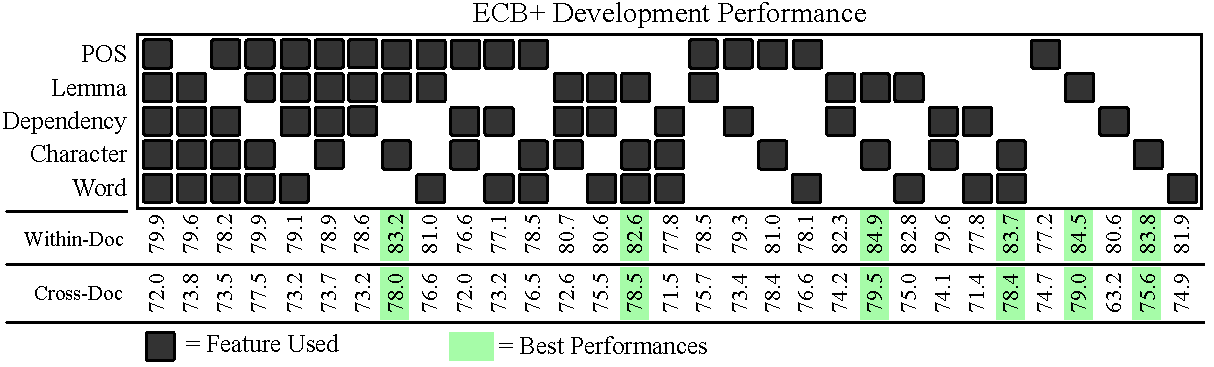
\includegraphics[width=0.82\textwidth]{graphics/features.pdf}
	\caption{The CoNLL F1 performance of our flagship CCNN + Neural Clustering system, using all combinations of features.}
	\label{fig:allfeatures}
\end{figure*}

We were interested in the five common, non-relational embedding features which are detailed in Section \ref{sec:features}: POS, Lemma, Dependency Lemma, Character, Word.  We tested all combinations of features on the Dev Set, and Lemma + Character Embedding yielded the best dev results (see Figure \ref{fig:allfeatures}).  Thus, our CCNN + Neural Clustering system used only these two features in its evaluation against other systems (see Table \ref{tab:others}).  

Our immediate evaluation measures the pairwise mention predictions.  As shown in Table \ref{} [TODO: make table], our CCNN model ourperforms the FFNN, SVM, and SameLemma baselines.

The final coreference results show that our CCNN model outperforms a FFNN, and that our Neural Clustering outperforms Agglomerative Clustering.  Figure \ref{} shows an example of where the aforementioned weaknesses of Agglomerative are improved by NC. [TODO: add figure demonstrating AGG VS NC examples.]  Further, when training and testing on gold mentions, we achieved CoNLL F1 scores of \textbf{81.2} and \textbf{72.4} for within-document and cross-document, respectively.  We denote these scores as the new baseline to which to compare future systems.

\begin{table*}[h]
\centering
\tabcolsep=0.15cm
\begin{tabular}{r|ccc|c|ccc|c|}
\cline{2-9}
& \multicolumn{4}{|c|}{Within-Document} & \multicolumn{4}{|c|}{Cross-Document}\\
\cline{2-9}
& \multicolumn{1}{c}{MUC} & B$^3$ & CEAF & CoNLL F1 & \multicolumn{1}{c}{MUC}& B$^3$ & CEAF & CoNLL F1\\
\hline
 \multicolumn{9}{|c|}{Test Set: ECB+ Gold Mentions} \\
 \hline
 \multicolumn{1}{ |c| }{SameLemma}& 58.3 & 83.0 & 75.9 & 72.4 & 84.2 & 68.2 & 48.0 & 66.8 \\
\multicolumn{1}{ |c| }{FFNN+AGG} & 59.9 & 85.6 & 78.4 & 74.6 & 77.7 & 69.9 & 50.1 & 65.9\\
\multicolumn{1}{ |c| }{FFNN+NC} & 60.7 & 86.7 &  79.4 & 75.6 & 74.9 & 67.8 & 56.3 & 67.0\\
\multicolumn{1}{ |c| }{CCNN+AGG} & 70.5 & 89.1 & 83.5  & 81.0 & 84.1 & 70.7 & 55.5 & 70.1\\
\multicolumn{1}{ |c| }{\textbf{CCNN+NC}}& 70.9 & 88.9 & 83.6 & \textbf{81.2} & 86.4 & 71.7 & 59.1 & \textbf{72.4}\\
\hline
\hline
 \multicolumn{9}{|c|}{Test Set: HDDCRP's Predicted Mentions} \\
 \hline
\multicolumn{1}{ |c| }{SameLemma}& 40.4 & 66.4 & 66.2 & 57.7 & 66.7 & 51.4 & 46.2 & 54.8 \\
\multicolumn{1}{ |c| }{HDDCRP}& 53.4 & 75.4 & 71.7  & 66.8 & 73.1 & 53.5 & 49.5 & 58.7\\
\multicolumn{1}{ |c| }{\textbf{CCNN+NC}} & 54.0 & 75.5 & 72.2  & \textbf{67.2} & 71.3 & 57.0 & 49.6 & \textbf{59.3}\\
 \hline
\hline
 \multicolumn{9}{|c|}{Test Set: Choubey's et. al. Mentions} \\
 \hline
\multicolumn{1}{ |c| }{SameLemma}& 48.8 & 66.7 & 65.1 & 60.2 &  68.1 & 53.3 & 47.2 & 56.2\\
\multicolumn{1}{ |c| }{Choubey}& 62.6 & 72.4 & 71.8  & 68.9 & 73.4 & 80.4 & 56.5 & 63.6\\
\multicolumn{1}{ |c| }{\textbf{CCNN+NC}} & 67.3 & 73.0 & 69.5  & \textbf{69.9}& 77.0 & 56.3 & 60.2 & \textbf{64.5}\\
 \hline
\end{tabular}
\caption{Comparison against other systems, while our models use only the Lemma + Character Embedding features.  FFNN denotes a Feed-Forward Neural Network Mention-Pair model.  AGG denotes Agglomerative Clustering.}
\label{tab:others}
\end{table*}

\textbf{Lemma Embeddings} were the most useful feature, followed closely by Character Embeddings.  Since \textit{SameLemma} has historically been a strong baseline, this is unsurprising.  

\textbf{Character Embeddings} were effective for the same reason String Edit Distance is often a strong feature: there tends to be a direct correlation between the textual similarity of mentions and their likelihood of being co-referent. Both random character embeddings and pre-trained ones yielded the same performance, suggesting that the power comes from the uniqueness of characters, not any \textit{meaning} conveyed in the characters.

Empirically, Lemma + Character Embeddings are complementary features; the semantic information conveyed within the lemma embeddings complement the syntactic information of character embeddings.  Related, POS by itself was a poor feature, but combining it with either Lemma or Character Embeddings offered strong results. 

Ideally, a classifier should learn how to combine all features such that the unhelpful ones are given no weight.  However, in practice, that is often extremely difficult, due to both the large parameter space and high entropy wherein some combinations of features seem to equally help as much as hurt.  Thus, we conclude that one should try to use the fewest features as possible for coreference resolution, then expand appropriately.

In all experiments, our results were inversely correlated with the amount of context our CCNN used.  That is, our best performance came when we used no context, only the mention words.  This agrees with the Choubey's, et. al. findings \cite{Choubey2017EventCR}.

\subsection{Comparison to Others' Systems}
\textit{SameLemma} has historically proven to be a strong baseline.  That is, anytime two mentions have identical lemmas, simply mark them as being co-referent.

Using the same mentions that were used by the HDDCRP and Choubey (Iteratively-Unfolding) systems, our flagship CCNN+NC system yielded the highest results, despite using few features.


\subsection{Error Analysis}
\textbf{False Positives} include mentions which are textually identical but not actually co-referent (e.g., \textit{placed} and \textit{placed}, which only differ in their direct objects).
\textbf{False Negatives} include abbreviations (e.g., \textit{i.r.} and \textit{injured reserve}) and colloquial phrases (e.g., The \textbf{casting} of Smith; (2) Smith \textbf{stepped into} the role; (3) was \textbf{handed the keys}).

[TODO: show actual examples]

Since our cross-document system relies on the within-document predictions, it is easy for errors to propagate.

\chapter{Proposed Work}
\label{sec:proposed}
\section{Joint Entity and Event Coreference}
\section{Motivation}
As shown in Figure [TODO: INSERT FIGURE], two sentences which contain co-referring entity mentions may also contain co-referring event mentions in a parallel fashion.  Table [TODO: CALCULATE STATS] demonstrates how often this occurs in the ECB+ corpus.  Since evidence of co-referring events increases the likelihood that the entities should also co-refer, we are motivated to model both entities and events, and to allow each model to influence the other.

% TODO: insert figure
\section{Related Work}
There has been some research which demonstrates benefits of jointly resolving mentions across multiple entities [TODO: cite the papers (p490 of Jurafsky)].  However, there has not been much research that uses event information to resolve entities.  Haghighi and Klein \cite{Haghighi:2010:CRM:1857999.1858060} include a feature which concerns the governor of the head of nominal mentions (which could be events).  Rahman and Ng \cite{Rahman:2011:CRW:2002472.2002575} uses the semantic roles of entity mentions, along with the verb pairs of their predicates.  These models use event information to help inform entity coreference; yet, they do not perform event coreference or use resolved events to inform entity coreference.

Choubey, et. al. \cite{Choubey2017EventCR} performs event coreference resolution via a feed-forward neural network.  Afterwards, in an ad hoc fashion, their system [TODO: describe their system]

Most similar to our proposed work, Lee, et. al. \cite{Lee:2012:JEE:2390948.2391006} [TODO: describe their system and mention that they use their own corpus, EECB, not ECB+]

%perform entity resolution via the Stanford Core NLP Toolkit.  Afterwards, all extracted event mentions are merged agnostically.  That is, the fact that they are events is ignored, and they could be merged with either pre-existing entity clusters or other event mentions.  Naturally, events merge with other events, since their properties are much different than entities.  So, even though their model allows for mixing entities and events, the confidence of one does not affect the confidence of the other.
\section{Approach}
We aim to first use strong entity coreference system.  We will evaluate both (1) our CCNN approach; and (2) Stanford Core NLP Toolkit's software on 3 different entity-labelled corpora:
\begin{itemize}
\item CoNLL-2012 Shared Task
\item EECB (the corpus developed in \cite{Lee:2012:JEE:2390948.2391006})
\item ECB+
\end{itemize}

\subsection{Semantic Trees}
Hopefully our CCNN approach outperforms Stanford's.  If it is reasonably close, we will work on refining our model.  Alternatively, I am interested in exploring semantic Tree-Based approaches, such as Tree-LSTM, and modelling the likelihood that two mentions' co-referring based on the similarity of their semantic trees.  That is, one could learn common mappings that occur, such as the example in Figure \ref{fig:dep_mapping} [TODO: make a figure to show two dependency trees].  A simple baseline could be Tree-Edit distance.  More involved approaches include:
\begin{itemize}
\item seq2seq model (where the Tree is expanded to linear form)
\item CNN model which learns patterns of sub-regions of trees
\item ensemble of auto-encoders, each of which calculates the cost of mapping from one sub-region to another ($||f(Tree(m_{1})) - f(Tree(m_{2})))||$)
\end{itemize}

\subsection{Joint Work}
We will use whichever model above that gives the best results on the 3 corpora.  Here, the emphasis of our research is not so much on developing the best possible entity coreference system, but to research the potential benefits from the joint modelling with events and to build each up in an iterative fashion.  Our goal is to use a Expectation-Maximization (EM)-style approach.  As a rough sketch (the math needs work and is not correct as is), we will aim for a back-and-forth like equations \ref{eq:em1} and \ref{eq:em2}.

\begin{equation}
\label{eq:em}
\begin{split}
P(m_{ent1}|m_{ent2}) = \frac{Q(m_{ent1}|m_{ent2}) + P(m_{event1}|m_{event2})}{\sum\limits_{m_{enti}}[Q(m_{enti}|m_{ent2})+ P(m_{eventi}|m_{event2})]} \\
\text{where} \hspace{2mm}
Q(m_{ent1}|m_{ent2}) = \frac{CCNN(m_{ent1}|m_{ent2})}{  \sum\limits_{m_{enti}} CCNN(m_{enti}|m_{ent2})  }
\end{split}
\end{equation}

\begin{equation}
\label{eq:em}
\begin{split}
P(m_{event1}|m_{event2}) = \frac{Q(m_{event1}|m_{event2}) + P(m_{ent1}|m_{ent2})}{\sum\limits_{m_{eventi}}[Q(m_{eventi}|m_{event2})+ P(m_{enti}|m_{ent2})]} \\
\text{where} \hspace{2mm}
Q(m_{event1}|m_{event2}) = \frac{CCNN(m_{event1}|m_{event2})}{  \sum\limits_{m_{eventi}} CCNN(m_{eventi}|m_{event2})  }
\end{split}
\end{equation}

\section{Comprehensive Coreference: Mention Detection + Coreference}
\section{Motivation}
Currently, Mention Detection (e.g., Event Detection aka Named Entity Recognition) has always remained a disjoint line of research from coreference resolution, despite the fact that the input of coreference resolution has always been the output of mention detection.  Naturally, the performance of mention detection affects the eventual performance of coreference.  Thus, it seems likely that merging these two into a single model could improve results, especially if one considers that (1) the confidence of two mentions co-referring could help estimate if the mentions are even valid mentions (e.g., ``ran in the'' should have low probability of corefering with any other mention, signifying that it is probably not a valid mention), and; (2) the confidence of a given text being a mention could help determine if two candidate mentions co-ref (e.g, ``Barack Obama will'' having a mention detection score of 0.5 and ``Barack Obama'' having a score of 0.95).
\section{Related Work}
Recently published \cite{D17-1018} was the very first work which uses this idea.  In short, the authors present the first end-to-end coreference model, whereby they consider all possible mention spans, and prune them based on boundaries learned from context during training.  Notably, the model does not use third-party syntatic parse information.  Instead, the only specific features used are: speaker, genre, span distance, mention width.  Note, their work was for entity coreference and they used the CoNLL-2012 shared task, as opposed to our ECB+ corpus which does not have speaker or genre information.

\section{Approach}
A notable difference between our proposed work and the related work \cite{D17-1018} is that we:
\begin{enumerate}
\item Want to consider \textit{all} mention spans as candidates, and calculate coreference predictions with them, as opposed to pruning them before coreference.
\item Predict the mention \textit{type} (e.g, action\_occurrence, person, organization, etc) along with each span, in attempt to help coreference
\item Want to perform both entity and event resolution, as described in the previous section
\item Want to perform cross-document coreference, not just within-doc
\end{enumerate}

The biggest challenge of these is arguably the $1^{st}$ item, as it is potentially prohibitely-expensive to compute all combination of candidate mention pairs, as this is $O(N^{4})$.  Current rough ideas for ways to approach this include:
\begin{itemize}
\item quick hashing techniques (e.g., MinHashing/LSH embeddings)
\item heuristics (alpha-beta pruning) to stop exploring longer mention spans which have low scores from their constuite unigram, bi-gram candidate mentions
\item try all mentions if possible (documents are short for the ECB+ corpus, so it might be possible, especially with parallel GPU jobs)
\end{itemize}

Specifically, I plan to evaluate our performance on (1) ECB+ corpus, as it has both entities and events labelled, and; (2) CoNLL-2012 for just entities, which will not leverage event coreference, as the corpus lacks this information, but it will give us a good comparison since this is the canonical corpus for entity coreference.

%\chapter{Conclusion}
%\section{Conclusion}
\backmatter % PROPOSAL
\bibliographystyle{plain}
\bibliography{proposal}
\end{document}
